\subsection{A one-feature rule}\label{sec:rule}

If the gain is in the primitive and its leaf, the practical question is whether every cloud needs its own search or whether a fixed rule captures the gain. Table~\ref{tab:rule} answers it on the \nRuleCells{} searched clouds. The reference is the \emph{per-cloud best}, the fastest single structure found on each cloud's search half; a rule's \emph{regret} is the latency of the structure it picks over that best. Every rule picks from the 55 tuned structures and is fitted leave-one-scene-out: when a cloud is scored, every cloud of the same scene at every size is left out of the fit, so a rule never sees the cloud it is judged on. Two latency columns are reported, the instrumented pass and the mean of the timed passes, because the two rank close variants differently and a rule should not depend on which one is read.

\begin{table*}[t]
\centering\footnotesize
\caption{Fixed rules against the per-cloud best (the fastest single structure on the search half), \nRuleCells{} searched clouds, fitted leave-one-scene-out. Regret is the geometric mean of the rule's latency over the best's; p90 its 90th percentile; the last column counts clouds where the rule is more than 15\% off. Left: the instrumented pass; right: the timed passes.}
\label{tab:rule}
% generated by scripts/paper/tables.py; do not edit
\begin{tabular}{lrrrrrr}
\toprule
Rule & regret & p90 & cells $>1.15$ & regret & p90 & cells $>1.15$ \\
\midrule
library octree default, leaf 32 & 1.746 & 2.18 & 68 & 1.950 & 2.77 & 68 \\
library kd-tree default, leaf 32 & 1.630 & 1.98 & 67 & 1.619 & 2.05 & 68 \\
floor: best of the 55 tuned singles per cell & 1.011 & 1.05 & 0 & 1.010 & 1.04 & 0 \\
one global schema & 1.067 & 1.21 & 10 & 1.074 & 1.18 & 12 \\
one schema per scan group & 1.078 & 1.23 & 12 & 1.106 & 1.33 & 14 \\
one split on the flatness score & 1.043 & 1.10 & 2 & 1.076 & 1.20 & 12 \\
\bottomrule
\end{tabular}

\end{table*}

\begin{figure}[tb]
\centering
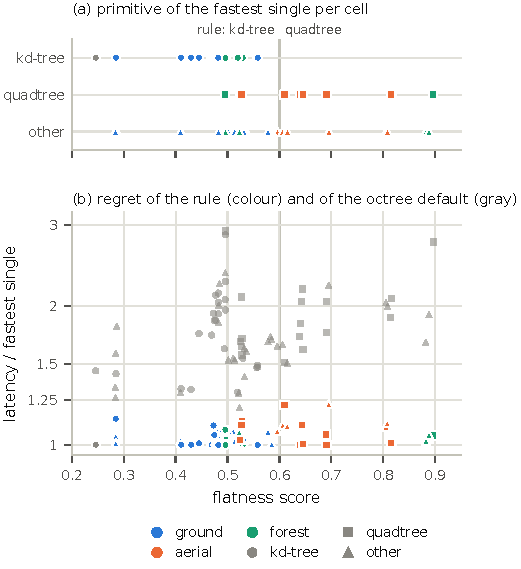
\includegraphics[width=\linewidth]{figures/fig_rule}
\caption{(a) The primitive of each cloud's fastest structure on the search half against the cloud's flatness score; the vertical line is the rule's split. (b) The regret of the one-split rule (coloured by scan group) and of the octree default (gray) per cloud. Marker shape: the primitive of the fastest structure.}
\label{fig:rule}
\end{figure}

The library defaults are the floor of the comparison: the octree default is \octreeDefaultRegret$\times$ the per-cloud best in the instrumented column and \octreeDefaultRegretTimed$\times$ in the timed one, the median kd-tree default \kdDefaultRegret$\times$, and every cloud but one is more than 15\% off. The ceiling is the best of the 55 tuned structures per cloud, at \floorRegret: the grid is dense enough that a search over it loses almost nothing to the open-ended genetic search. One global structure, the same for every cloud, is \globalSchemaRegret$\times$ the per-cloud best: a 48-level sliding-midpoint kd-tree with a leaf of 64 or 128 points, which is already most of the way. One structure per scan group does worse (\groupSchemaRegret), because the forest group mixes a flat park, where a quadtree wins, with a volumetric forest, where a kd-tree does.

The rule that works is a single split on one feature. A regression tree of depth one over thirteen cloud features (point count, density, aspect ratios, height statistics, covariance shape, occupancy, verticality and flatness) chooses the \emph{flatness score} in every fold, with the same threshold in both latency columns:
\[
\text{flatness} = \bigl(1 - \tfrac{\text{z extent}}{\max(\text{x extent}, \text{y extent})}\bigr)\cdot\tfrac{\text{planarity} + 1 - \text{scattering}}{2},
\]
from the extents of the cloud and the covariance eigenvalues of a fixed-seed sample of its points. Below 0.60 the rule picks the sliding-midpoint kd-tree with 48 levels and leaf 128; above it, a quadtree with 16 levels and a leaf of 64 to 128. Its regret is \ruleRegret{} in the instrumented column and \ruleRegretTimed{} in the timed one, with a 90th percentile of \ruleRegretP{} and \ruleCellsOver{} clouds more than 15\% off. In log terms the rule closes \ruleCapturePct\% of the distance from the octree default to the per-cloud best; what the search adds on top, four to eight percent, is about the measurement noise of the per-cloud best itself, which is the minimum over some 120 noisy candidates whose repeat coefficient of variation is several percent. A tree of depth two fits no better and picks a different second feature in each fold: with sixteen scenes there is nothing more to learn.

Figure~\ref{fig:rule}a shows why one feature suffices. The score separates the 2.5-dimensional scenes, the aerial terrain and cities and the park, where the fastest structure is a quadtree, from the three-dimensional ones, the ground scans and the forests, where it is a kd-tree. The one scene the rule misplaces is a UAV terrain survey whose score of 0.53 falls on the kd-tree side, and that scene is most of the aerial regret in Figure~\ref{fig:rule}b. On every other cloud the rule is within a few percent of the per-cloud best, where the octree default is between 1.3 and 3 times off.

Two caveats bound the claim. The rule was fitted and scored on the search half; on the clouds where its pick, or a structure with the same primitive, leaf and depth, happened to be among the finalists timed on the held-out half, it is within a fraction of a percent of the best timed structure there, but that sample is biased towards clouds where the rule's pick was already a finalist. And the leaf capacities it names were measured on 4\,KiB pages; Section~\ref{sec:ram} shows that the optimum moves on a machine with transparent huge pages enabled.
